%%%%%%%%%%%%%%%%%%%%%%%%%%%%%%%%%%%%%%%%%%%%%%%%%%%%%%%%%%%%%%%%%%%%%%%%%%%%%%%
%                         File: osa-revtex4-1.tex                             %
%                        Date: April 15, 2013                                 %
%                                                                             %
%                              BETA VERSION!                                  %
%                   JOSA A, JOSA B, Applied Optics, Optics Letters            %
%                                                                             %
%            This file requires the substyle file osajnl4-1.rtx,              %
%                   running under REVTeX 4.1 and LaTeX 2e                     %
%                                                                             %
%                   USE THE FOLLOWING REVTeX 4-1 OPTIONS:                     %
% \documentclass[osajnl,twocolumn,showpacs,superscriptaddress,10pt]{revtex4-1}%
%                    %% Use 11pt for Applied Optics                           %
%                                                                             %
%               (c) 2013 The Optical Society of America                       %
%                                                                             %
%%%%%%%%%%%%%%%%%%%%%%%%%%%%%%%%%%%%%%%%%%%%%%%%%%%%%%%%%%%%%%%%%%%%%%%%%%%%%%%

%\documentclass[osajnl,twocolumn,showpacs,superscriptaddress,10pt]{revtex4-1} %% use 11pt for Applied Optics
\documentclass[osajnl,preprint,showpacs,superscriptaddress,12pt]{revtex4-1} %% use 12pt for preprint option
\usepackage{amsmath,amssymb,graphicx}
\usepackage{multirow}
\usepackage{setspace}
\usepackage{longtable}

\newcommand{\procspie}{{Proc. ~SPIE}}
\begin{document}

\title{Characterization of gaps in directly bonded Si compound optics}

\author{Michael Gully-Santiago}\email{gully@astro.as.utexas.edu}
\author{Daniel T. Jaffe}
\affiliation{Department of Astronomy, The University of Texas at Austin, Austin, TX, 78712, USA}

\author{Victor White}
\affiliation{NASA Jet Propulsion Laboratory, Pasadena, CA}


\begin{abstract}
Si direct bonding offers flexibility in the design and development of large Si optics.  The bonding process presents challenges in meeting the performance demands and physical robustness, in particular for cryogenic and space applications.  Air cavities in between the Si interface will have large Fresnel reflections which will interfere as a low-Finesse Fabry-P\`erot etalon.  Even small (35 nm) gaps reduce transmission through a direct bonded Si compound optic by 5\% at $\lambda = $ 1.15 $\mu$m at normal incidence.  Stock near infrared spectrophotometers like the Cary5000 from Agilent offer 0.2\% photometric precision.  We can use instruments like the Cary 5000 to detect and measure gaps as small as 8 nm by measuring transmission as a function of wavelength.  Our approach involves modeling multiple incoherent reflections within the substrate interfaces with a wave transfer matrix, modified for intensities rather than complex amplitudes.  The detection and morphology of minuscule gaps provides valuable feedback in the design of Si direct bonding strategies.
\end{abstract}

\ocis{(030.1670) Coherent optical effects; (050.2230) Fabry-Perot; (120.2230)   Fabry-Perot; (120.2830) Height measurements; (120.4610) Optical fabrication; (120.7000) Transmission; (120.7000)   Transmission; (220.4840) Testing; (230.4170) Multilayers; (240.1485) Buried interfaces;  (300.6340) Spectroscopy, infrared; (310.6628)  Subwavelength structures, nanostructures}

\maketitle %% required

\section{Introduction}


Direct optical bonding of silicon allows manufacturers to combine Si parts with no Fresnel loss at the interface.  The high refractive index of Si makes this advantage particularly useful.  Traditional figures of merit for the optical audits of bonds, however, are either insensitive to gaps that are small yet have a significant impact on throughput and phase coherence, or do not provide quantitative information about the extent of the gaps along the direction of propagation.

%Issues with the quality of the bonds become particularly acute when the optics are used in double-pass and/or when the incidence angle at the bonds is far from the normal.  

The University of Texas diffractive optics group produces diffraction gratings on silicon using microlithographic techniques \cite{1998SPIE.3354..201J,2010SPIE.7739E.146W}.  These gratings are used either in transmission (i.e. as grisms \cite{2008SPIE.7014E..77D, 2010SPIE.7739E.123G}), or in reflection (i.e. as immersion gratings, \cite{2007ApOpt..46.3400M, 2010SPIE.7739E.146W,2012SPIE.8450E..2SG}.  These gratings operate throughout the infrared, from 1.2 to 38 $\mu$m, and find application in ground-based (IGRINS \cite{2010SPIE.7735E..54Y, 2012SPIE.8450E..2SG}), airborne (SOFIA FORCAST \cite{2008SPIE.7014E..77D}), and space (JWST NIRCAM \cite{2005SPIE.5904...21B,2010SPIE.7739E.123G}) applications.  To date, our group has produced the gratings on large (up to 100 mm diameter and 30 mm thick) monolithic pieces of monocrystalline silicon and we shape the substrates by sawing, grinding, and polishing to form the final devices \cite{2010SPIE.7739E.146W}.  The next generation of astronomy and earth science spectrographs, however, will need optical devices larger and more precise than what can be made with existing technology.  The proposed Giant Magellan Telescope \cite{2012SPIE.8444E..1HJ} Near Infrared Spectrograph \cite{2006SPIE.6269E.143J,2010SPIE.7735E..87L} (GMTNIRS) will need immersion gratings with thicknesses up to 60 mm and lengths up to 200 mm.  Substrates of the required size cannot fit into conventional processing equipment like reactive ion etchers and electron-beam lithography tools.  Large, thick Si substrates are also prohibitively expensive to experiment on.  Silicon direct bonding \cite{1986JAP....60.2987S,2012SPIE.8450E..2TV} offers advantages by allowing us to produce the diffraction grating on a thin (0.5$-$10 mm) low-mass Silicon wafer or puck that can later be bonded to a fine polished Si prism substrate.  Other groups producing Si diffractive optics are also experimenting with or using this approach (see \cite{2012SPIE.8450E..2TV} and \url{www.lumella.com}).


While it is possible that proper precautions can be made to eliminate all micron-sized particles from both Si surfaces prior to bonding, the power-law particle size distribution in clean-room environments \cite{doi:10.1080/02786828608959094} means that it is significantly more difficult to assure that no particles of the 10$-$60 nm size scale are present.  Small particles could be a concern if they act as ``tent poles", that create gaps where the bonding is incomplete (Figure \ref{figParticle}).  Some authors \cite{1991JaJAP..30..615M, 1992JEMat..21..669M, 1989JaJAP..28L2141L, Mitani1990} have referred to large ($\sim$ 1 $\mu$m size) gaps as \emph{IR bubbles}, or simply bubbles, owing to their appearance in infrared (IR) transmission images as contiguous regions of a deficit of IR transmission.  The gaps have also been referred to as voids\cite{2000RScI...71.1869G}, interfacial voids, or gaps.  In this paper we will reserve the term ``IR bubbles'' for gaps that are large enough to be detected directly in conventional IR imaging.  The term ``gap'' will apply more broadly to any finite size gap.

Finite gaps will degrade the performance of a final device, either through optical aberrations or transmission loss.  The effect of the gap size on the IR transmission is the topic of this paper.  The effect of the gap on optical aberrations is beyond the scope of this paper.  

A gap might also degrade the mechanical integrity of a final compound optic.  In practice, the part must survive thermal shocks and shake tests.  The gap size scales we can probe with our optical technique are comparable to the range over which molecular (van der Waals) forces are acting.  It is conceivable that the strength of the bond energy can be constrained from the \emph{in situ} measurement of the separation and that therefore our optical technique can provide not only a measure of the transmission but also an indication of the mechanical robustness of the bond.  By measuring both the spatial and axial extent of any gaps, the new metrology technique informs revisions of the bonding strategy that can improve both the optical and mechanical performance.  We do not investigate the mechanical robustness further.  

There are two main solutions for reducing risk attributable to gaps.  The first approach is to prevent gaps from forming in the first place, specifically by removing all possible contaminants from the environment before bonding.  Typically this approach involves disciplined handling protocols, and rigorous multi-stage cleaning steps.  The reason the approach is so hard is that hydrocarbons can serve as catalysts for gap formation\cite{1991JaJAP..30..615M}, and that these hydrocarbons are common in Si wafer handling equipment.  Unconventional micro-cleanroom approaches have been effective at meeting the goal of bubble-free bonding\cite{1989JaJAP..28L2141L}.  The second approach is to accept the likelihood that gaps will occur, and take steps to remove them.  The most cited way to get rid of gaps is to anneal them\cite{Mitani1990}.  We describe the current understanding of both approaches in Section \ref{secHistory}.

Whatever technique one uses to remove or reduce the effects of gaps, it is essential to have a quantitative method by which to assess accurately the optical impact of the gaps before and after treatment.  This paper introduces a technique for directly measuring gaps at silicon-silicon interfaces.  Mitani and G\"oselle review other techniques for measuring and mapping gaps\cite{1992JEMat..21..669M}.  One key technique is identifying IR Newton rings from IR imaging\cite{Mitani1990}.  The number and morphology of Newton rings yields information about the lateral and axial extent of large gaps. Specifically, dark-light fringes manifest when the gap is comparable to the vacuum wavelength or larger.  Our technique is IR interference in the limit of small gaps down to 20 nm or less.  

There are other techniques for mapping gaps.  X-ray topography \cite{1992JEMat..21..669M,1994JaJAP..33....6H} exploits the change in optical density along lines of sight to allow precise high spatial resolution measurements of the spatial extent of gaps with axial dimensions as small as a few nanometers.  In ultrasound microscopy, the density change at the gap interface produces reflections of sound waves and enables mapping the lateral gap dimensions but produces limited information about the axial dimension \cite{2000RScI...71.1869G}.  

Here we describe an application of the IR interference technique with new precision instrumentation in the near infrared to measure the axial extent of gaps at the few nanometer size scale.  In this paper we show that gaps as small as 35 nm cause an unacceptable degradation in transmission performance.  


\section{History of Si direct bonding}
\label{secHistory}

The foundation paper on Si bonding came in 1986\cite{1986JAP....60.2987S}.  After that, there was a sequence of papers using IR imaging to look for evidence of defects in the bond.  \cite{1988JaJAP..27L2364S, 1995ApPhL..67.3614G} directly monitored the bond propagation with IR imaging.  \cite{1988JaJAP..27L2364S, 1989JaJAP..28L2141L} demonstrated gap-free bonding in a micro-cleanroom, in which the bonding process occurs immediately after a rinse-spin-vacuum cycle inside of a vacuum enclosure.  Our group has not attempted the micro-cleanroom technique owing to the challenge of spin-cleaning large (30 mm thick) Si substrates.  It is not clear whether the custom micro-cleanroom technique has gained wide usage.  \cite{1989JaJAP..28L2141L} directly measured the bond surface energy.  \cite{Mitani1990} discussed the causes and remedies for bubble formation.  Specifically, the IR bubble density changes as a function of anneal temperature\cite{1992JEMat..21..669M}, with bubbles disappearing at temperatures greater than 1100$^\circ$ C.  The chemistry of the bonding interface began to be understood with infrared absorption spectroscopy and multiple internal reflection spectroscopy\cite{feijoo1994}, which lent credibility to the idea of distinct temperature phases and evidence for Si$-$H bonds\cite{1995ApPhA..61..101R}.  A robust picture of the chemistry as a function of anneal temperature was ultimately fleshed out\cite{1996JaJAP..35.2102R, 1998AnRMS..28..215G}.  Other variables potentially affecting bond strength were studied, for example surface roughness\cite{JJAP.37.4197}, surface topography \cite{2001JOptA...3...85G}, surface preparation\cite{1996ApPhL..68.2222T}, annealing time \cite{2000JAP....88.4404H}, ambient pressure and substrate thickness \cite{1995ApPhL..67..863G, 2007ApOpt..46.6793H}, and moisture and defects \cite{2001JAP....89.6013L}.  Notably, \cite{JJAP.37.4197} found that surface roughness above 1.3 nm RMS results in poor bonding quality in their sample of wafers etched with Argon.  Results from studies of surface topography are inconclusive\cite{2001JOptA...3...85G}.  Nowhere in the literature did we find a technique similar to the one presented here, probably because the technique relies on the high precision of relatively new IR capable spectroscopy that was not widely available until this decade.


\section{Conceivable pitfalls in Si-Si direct bonding}

\subsection{Particles}

\begin{figure}[htbp]
\centerline{\includegraphics[width=0.95\columnwidth]{figs/SiTentCatFig2.pdf}}
\caption{Schematic of a particle preventing bonding of two Si surfaces\label{figParticle}.  There are two conceivable scenarios in which particle contamination can cause gaps in the bond.  \emph{Left-} The particle serves as a mechanical structure hindering the Si-Si bond from zippering up.  The geometry is like a tent-pole.  \emph{Right-} The particle serves as a catalyst for gas formation.  There is evidence that hydrocarbons can serve as catalysts.  The especially pernicious particles are ``thermally unstable hydrocarbon contaminants on the surfaces coming from plastic containers or simply from the ambient in a cleanroom'' \cite{1998AnRMS..28..215G}. }
\end{figure}

There are two major conceivable pitfalls in Si-Si direct bonding.  The obvious pitfall is particle contamination.  Figure \ref{figParticle} shows a schematic of a particle wedged between two flat Si optical surfaces.  A single 0.6 $\mu$m particle can create a dark IR bubble from interference.  In a class 100 cleanroom, the particle volume density could be as high as $\rho=100$ particles/ft$^3$, for particle sizes larger than 0.5 $\mu$m.  What we care about is not the volume number density of particles, but the delivered surface flux $F=\rho(D) v(D)$, where $v(D)$ is the average freefall speed of particles, which is a function of particle size.  Figure 5 of Cooper 1986\cite{doi:10.1080/02786828608959094} shows the surface flux (particles cm$^{-2}$ s$^{-1}$) vs. particle size ($\mu$m).  There will be roughly $10^4$ times more 10 nm sized particles than 1 $\mu$m sized particles.  In other words:
$$\log(F) = -2\log(D) + const. \label{eqnParticleFlux}$$

For every obviously detectable IR bubble, there are thousands more particles that could unacceptably degrade the transmission performance.  One key idea that saves the day, is the intuition that the areal fill factor scales at least as fast as $D^2$.  Imagine that the particles serve as miniature tentpoles.  The volume beneath the tentpole looks like a cone.  Since the number density scales as roughly $D^{-2}$, (per the Equation \ref{eqnParticleFlux} above) the total area covered by particles might be constant in $log(D)$.  Simply put, the big particles cover just as much area as the small particles, even though there are many more small particles.  It is further conceivable that the areal fill factor attributable to a tent pole particle scales even faster than $D^2$ since surface energy probably scales inversely with distance of the pieces (\`a la VanDerWaals).  The small particles are even less of a problem than the large particles, since the small ($\sim10-60$ nm) particles will have lower average etalon reflectivity than larger (500-1000 nm) particles.  This last point will become clearer in later sections.

It has been shown\cite{1992JEMat..21..669M} that gases produced at the Si$-$Si interface seep along the interface surfaces.  Pressure builds around catalysts.  In this sense, the size of the particle causing a gap cannot be uniquely identified from observations of the extent of gaps.  In Section \ref{secResults} we address the question of the origin of gaps.  Specifically, are the particles more like \emph{tentpoles}, rigid structures that merely prevent the zippering up of the bond?  Or are the particles more like \emph{catalysts} so that their size is immaterial- the particles merely accelerate the production of gases that bow out the bond?  These are open questions.

\subsection{Surface roughness or large-scale non-conformance}
Another possible source of gaps at the bond is inherent roughness in the initial surfaces that leads to a failure to conform.  Stiff non-flat Si surfaces will not conform upon contact leaving the complement of the aberrations as an air gap. Unconventional thick ($\sim$ 30 mm) Si pucks are less conformal than wafers are, so we expect thick substrates could have gaps even in the absence of particles.  Most of our thick substrates are optically polished to less than 60 nm peak to valley over the 3 to 4 inch diameter clear aperture.  We assume that if enough pressure is placed on the substrates during bonding, then the surfaces will come in contact and zipper up.  Subsequent annealing will strength the bond.

\section{Si$-$Si Fabry P\`{e}rot measurement theory}
\label{secTheory}

\subsection{The Si$-$Si interface gap is a low Finesse Fabry-P\`{e}rot etalon}

Our measurement technique exploits the large Fresnel reflection \cite{2001opt4.book.....H} at the Si$-$vacuum interface.  The refractive index of silicon at room temperature ranges from 3.55$-$3.45 from $\lambda = $ 1150$-$2500 nm \cite{2006SPIE.6273E..77F}, one of the largest refractive indices of any conventional material.  The Fresnel reflection is about 30\% per surface.  For comparison, conventional optical materials with refractive indices in the range 1.5$-$1.7 have Fresnel reflection of merely 4$-$7\% per surface.  Figure \ref{figSiIndexFinesse} shows the refractive index as a function of wavelength for room temperature, which we computed using the coefficients from \cite{2006SPIE.6273E..77F}.

\begin{figure}[htbp]
\centerline{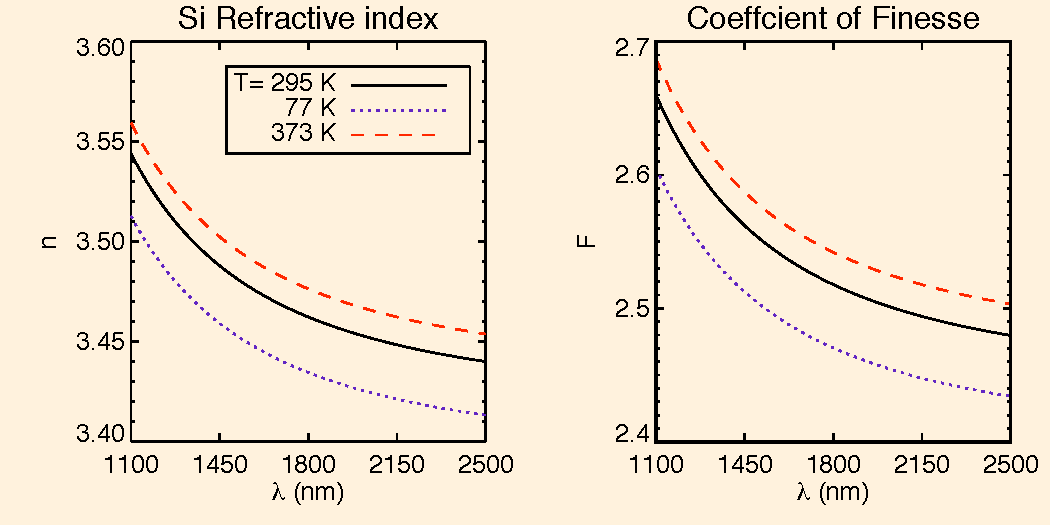
\includegraphics[width=0.95\columnwidth]{figs/SiIndexAOmgsFinesseFig.pdf}}
\caption{Plot of refractive index, $n$, and coefficient of finesse, $F$, as a function of wavelength, $\lambda$.\label{figSiIndexFinesse} We computed the temperature dependent refractive index from the tabulations of \cite{2006SPIE.6273E..77F}, and extrapolated past their upper temperature bound to estimate values near 373 K.  The coefficient of finesse is defined in Equation \ref{eq:FabPerot}.  The minuscule temperature dependence is largely negligible, and for the rest of the paper we assume room temperature refractive index.}
\end{figure}

The Si$-$Si interface gap is a low-Finesse Fabry-P\`{e}rot etalon\cite{2007fuph.book.....S}.  The transmission through a Fabry-P\`{e}rot depends on the wavelength of light, the reflectivity of the etalon sidewalls, and the size of the gap.  We assume transmission is at normal incidence, the refractive index of the gap is 1.0, and the material is at room temperature.  We compute the reflectivity for an Si$-$vacuum interface, which is a modest function of wavelength through the refractive index of Silicon, $n(\lambda, T)$ \cite{2006SPIE.6273E..77F}, as shown in Figure \ref{figSiIndexFinesse}.  In the equations ahead we drop the subscripts on the refractive index $n(\lambda, T) \rightarrow n$ and the coefficient of finesse $F(\lambda, T) \rightarrow F$ for clarity.  The computation is simply Fresnel's law at normal incidence:

\begin{eqnarray}
R = \frac{(n-1)^2}{(n+1)^2} \\
F \equiv \frac{4R}{(1-R)^2}
\end{eqnarray}

The reflectivity is about 30\% in the wavelength range 1100 to 5000 nm.  We've defined the coefficient of finesse\cite{2007fuph.book.....S}, $F$, a customary way to encapsulate the Fabry-P\`{e}rot etalon's dependence on the reflectivity.  The coefficient of finesse is shown in the right panel of Figure \ref{figSiIndexFinesse}.  Si is negligibly absorbing longward of about $\lambda$ = 1200 nm, which we verified by comparing the transmission of Si reference samples of different thicknesses, as shown in Figure \ref{figSiAbsorbfig}.  Figure \ref{figSiAbsorbfig} also verifies a key assumption that we will make when comparing the transmission of Si pucks of different heritage and thickness.  The Si refractive index is indistinguishable from sample to sample for the wavelength ranges we care about- the non-absorbing wavelengths greater than about 1200 nm.  \cite{2006SPIE.6273E..77F} cites the wide variety of values for refractive index from the literature as evidence that batch-specific Si should be used as reference for cases in which absolute accuracy greater than $\pm5\times10^{-3}$ is desired.  An absolute deviation of $\pm5\times10^{-3}$ in refractive index corresponds to a Fresnel transmission difference of about 0.2\%, which is comparable to our measurement uncertainty.  In the next subsection we work out the wavelength dependent transmission for the air etalon.

\begin{figure}[htbp]
\centerline{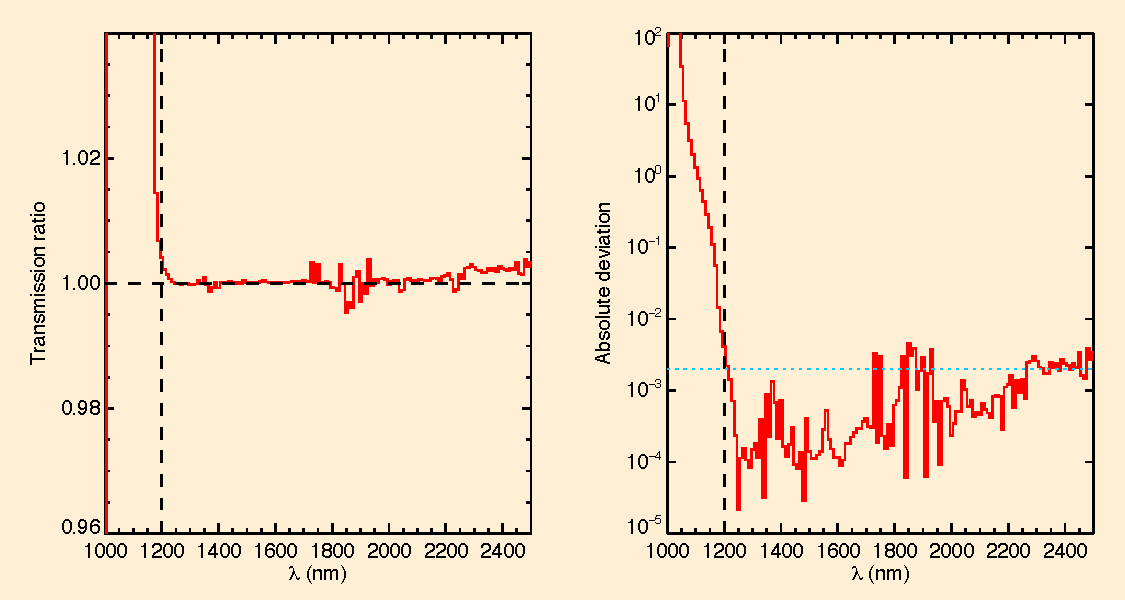
\includegraphics[width=0.95\columnwidth]{figs/fpAbsorbfig}}
\caption{Ratio of transmissions of Si wafers of different thicknesses, specifically the transmission of a thin ($\sim0.5$ mm) Si wafer divided by that of a 3 mm thick Si puck.  Both samples were double side polished.\label{figSiAbsorbfig}  The transmission scatters about 1.0 in wavelength ranges for which Si is negligibly absorbing for a path length ratio of $\sim$6, and exceeds 1.0 in wavelength ranges for which Si absorption is detected. The left panel shows that Si is firmly absorptive shortward of $\lambda \; =$ 1200 nm.  The right panel shows the absolute deviation from unity on a log scale.  The typical uncertainty and drift per measurement is about 0.2\%.  Absorption is detected at 0.4\% at $\lambda \;=$ 1200 nm.}
\end{figure}

\subsection{Predicted transmission spectrum for bonded Si with finite interface gap}
\label{secTheory}
There is a key hurdle in computing the transmission spectrum for bonded Si with a finite interface gap- multiple incoherent reflections occur within the Si substrate at normal incidence.  Treatments for multiple coherent reflections have been described in detail in the optics literature \cite{2007fuph.book.....S}.  The wave transfer matrix technique treats each dielectric interface as a matrix with elements relating the pre- and post- interface complex amplitudes in the left and right directions.  We adapted the wave transfer technique for incoherent interactions \cite{2002ApOpt..41.3978K}.  Specifically I constructed an incoherent wave transfer matrix whose elements relate the intensities (and not complex amplitudes) before and after an interface.  The details are worked out in Appendix \ref{sec:Append-IMRTMM}.  We computed the transmission for two scenarios- first a double side polished (DSP) Si puck with no gap, and second a pair of bonded Si pucks with a gap thickness $d$.  The DSP Si puck with no air gap has a transmission equal to:

$$
T_{DSP} = \frac{2n}{1+n^2} \label{eqnAbsDSPtrans} \\
$$

which has an average value of about 53\%.  Note that this transmission is above a na\"ive value of $T_{DSP}=(1-R^2)$, which does not take into account multiple incoherent reflections, and is therefore an underestimate.  Figure \ref{figAbsoluteTrans} shows a plot of Equation \ref{eqnAbsDSPtrans} in the wavelength range 1200$-2500$ nm.  If the Si wafer path thickness is less than the coherence length for the given spectral bandwidth, then the multiple reflections would interfere coherently, and the Si wafer would behave as a Fabry-P\`erot etalon.  This scenario is beyond the scope of this paper, since we are primarily interested in thick substrates with small gaps in between the interfaces.%We work out this behavior in the Appendix and show that in the limit $l>> \lambda^2 / \delta \lambda $ the spectral transmission tends to equation X.  

%The following 3 figures were made with fabry_perot_Si_20140421.pro and other variants.
\begin{figure}[htbp]
\centerline{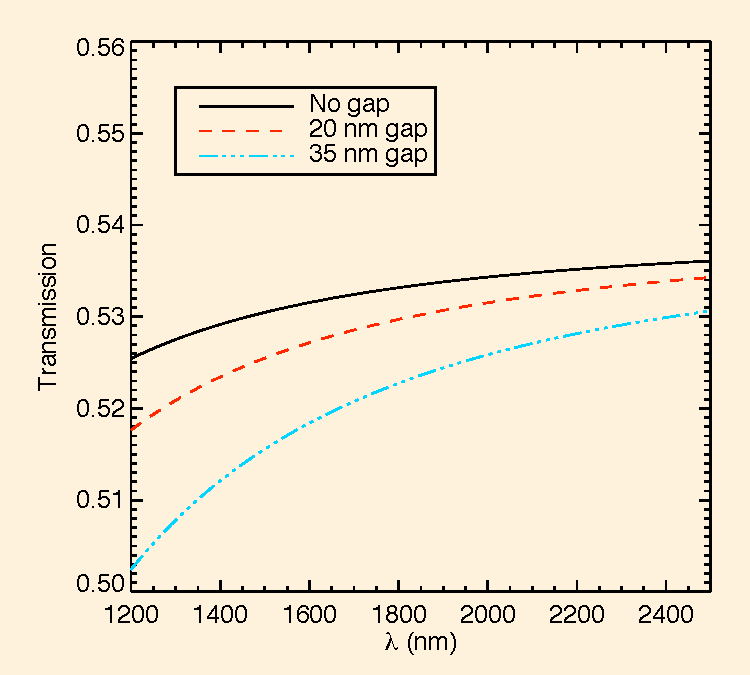
\includegraphics[width=0.65\columnwidth]{figs/20140421_absolute.pdf}}
\caption{Modeled absolute transmission through a silicon substrate with no gap (top black solid curve), and small gaps of axial extent 20 nm (red dashed curve) and 35 nm (cyan triple-dot dashed curve)\label{figAbsoluteTrans}.  The absolute transmission through Si depends on wavelength since the refractive index depends minutely on wavelength.  This curve is only accurate for normal incidence transmission.  Furthermore, the curve assumes the multiple reflections within the Si substrates add incoherently as discussed in detail in Appendix \ref{sec:Append-IMRTMM}.}
\end{figure}

\begin{figure}[htbp]
\centerline{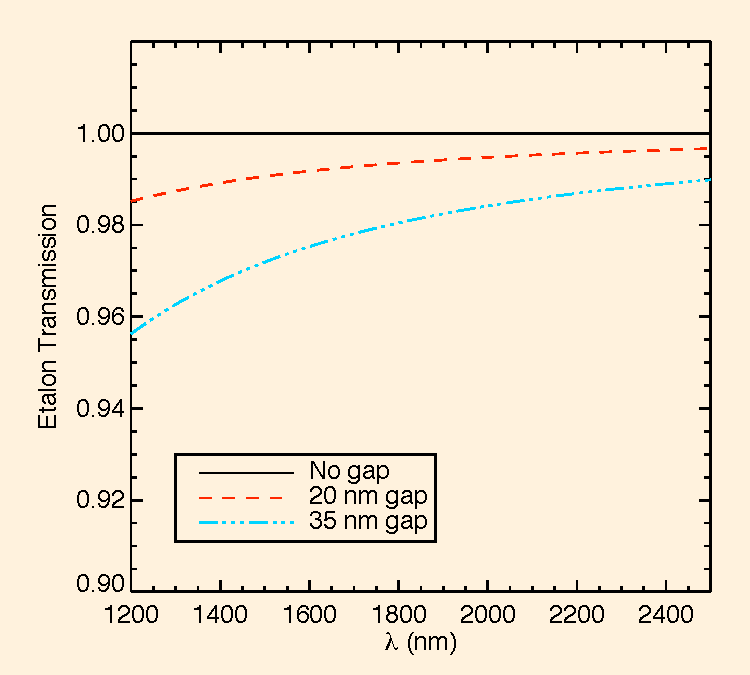
\includegraphics[width=0.65\columnwidth]{figs/20140421_absoluteB.pdf}}
\caption{Modeled etalon transmission through a silicon substrate with no gap (top black solid curve), and small gaps of axial extent 20 nm (red dashed curve) and 35 nm (cyan triple-dot dashed curve)\label{figEtalonRelTrans}.  The curves are examples from a family defined in Equation \ref{eqFP}.   The limit of no gap is 100\% transmissive, compared to a DSP reference.  A 35 nm gap degrades the transmission over a DSP reference by 4\% at 1200 nm.}
\end{figure}

Now consider a pair of bonded Si pucks with a gap thickness $d$. We derive the absolute transmission of bonded Si substrates with a gap in Equation \ref{eqn:Tetalon} in the Appendix.  We normalize the absolute transmission by the transmission with no gap to isolate the effect of the gap.  We call this normalized transmission the etalon transmission $T_{e}$, since it isolates the effect of the etalon on the transmission.

$$T_{e} = \frac{n^2+1}{2 n F \sin ^2(2\pi \frac{d}{\lambda})+n^2+1} \label{eqFP} \\$$

It is clear that in the limit $\lim_{d \rightarrow 0}$, the etalon approaches 100\% transmission.  Figure \ref{figEtalonRelTrans} shows a plot of Equation \ref{eqFP} for gap sizes, $d$, of 20 nm and 35 nm.  In Section \ref{secResults} we compare wavelength dependent transmission measurements to by-eye fits of Equation \ref{eqFP}.  

\begin{figure}[htbp]
\centerline{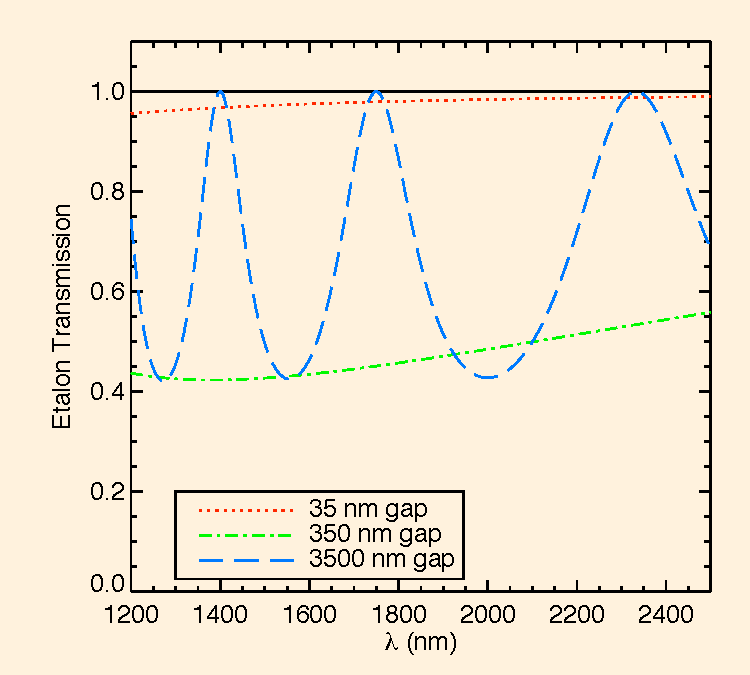
\includegraphics[width=0.65\columnwidth]{figs/20140421_absoluteC.pdf}}
\caption{Modeled etalon transmission through a silicon substrate with gaps of axial extent 35 nm (red dotted curve), 350 nm (green dash-dot curve), and 3500 nm (blue long-dashed curve)\label{figEtalonRelTrans}.  The curves are examples from a family defined in Equation \ref{eqFP}.  The 3500 nm gap curve has obvious Fabry-P\`erot fringes, whereas the 35 and 350 nm gap curves vary smoothly with wavelength.} 
\end{figure}

\section{Imbedding gaps of known sizes}

\begin{figure}[htbp]
\centerline{\includegraphics[width=0.95\columnwidth]{figs/VG03patternSchematic.pdf}}
\caption{Schematic of part VG03 \label{figVG03pattern}.  The 100 mm diameter VG03 is comprised of two 3.3 mm thick silicon pucks.  We patterned a 25 mm diameter hole on one of the pucks.  The depth was 4.0 $\mu$m as indicated by Dektak profilometry.  We also patterned a low-fill factor petal pattern surrounding the hole.  The purpose for these patterns was to have gaps of known dimensions against which we could test the optical metrology technique we describe in this paper.}
\end{figure}

We evaluated our metrology method by imbedding gaps of known sizes in the interface.  Here we describe the process of how we made the gaps and how we characterized their axial extent.  

The substrate thicknesses ranged from 0.5 to 3.3 mm per substrate.  We classify the 3.3 mm thick substrates as ``pucks'' and the $\sim$1.0 mm thick substrates as ``wafers''.  The distinction between the two classes of substrate thickness is based on the anticipation that thin substrates will conform more easily to their bonding partner substrates.  There is also evidence that bond front propagation is slower in thick pucks \cite{2007ApOpt..46.6793H} than in wafers.  

The three important characteristics of the gaps are their axial extent, their lateral areal extent, and their areal fill factor.  We bored holes in silicon with inductively coupled plasma etching.  We used two different gases with low and high etch rates.  CHF$_3$ on Si exhibited about 0.3 nm/second etch rate, SF$_6$ exhibited about 1 micron/minute.  The area exposed to the process gases was about 1 inch diameter circles, or 15 mm $\times$ 20 mm rectangles.  We protected the unexposed areas with thick photoresist.  We achieved etch depths of 15$\pm$5 nm and 4000$\pm$100 nm, as measured with Veeco NT9100 Optical Profiler for the small depth, and Dektak stylus profilometry for the large depth.  Table \ref{tabbondexper} has more information about the bonding samples, and Table \ref{tabPatternFills} lists the properties of the patterns.  The fill factor is defined as the pattern area covered by gaps relative to the total pattern area.  Figure \ref{figVG03pattern} shows a schematic of VG03 and its pattern, as described in Table \ref{tabbondexper}.  In a second round of experiments we achieved gap sizes of 14$-$95 nm on four substrates with three meshes with coarse, medium, and fine boxes, each with 50\% fill factors.  For measurements taken with the Veeco NT9100 Optical Profiler, uncertainties were constructed by inspecting the histogram of topology, as shown in Figure \ref{figVS20pattern}.  The large-scale distortions were removed from the topology by masking and flattening to ensure that the uncertainties accurately reflect the distribution of measured heights.  The stylus profiliometry measured values were simply assigned an uncertainty of 5\%, which was consistent with our intuition and experience.  Table \ref{tabbondexper} lists part numbers and descriptions for our bonded substrates.

\begin{figure}[htbp]
\centerline{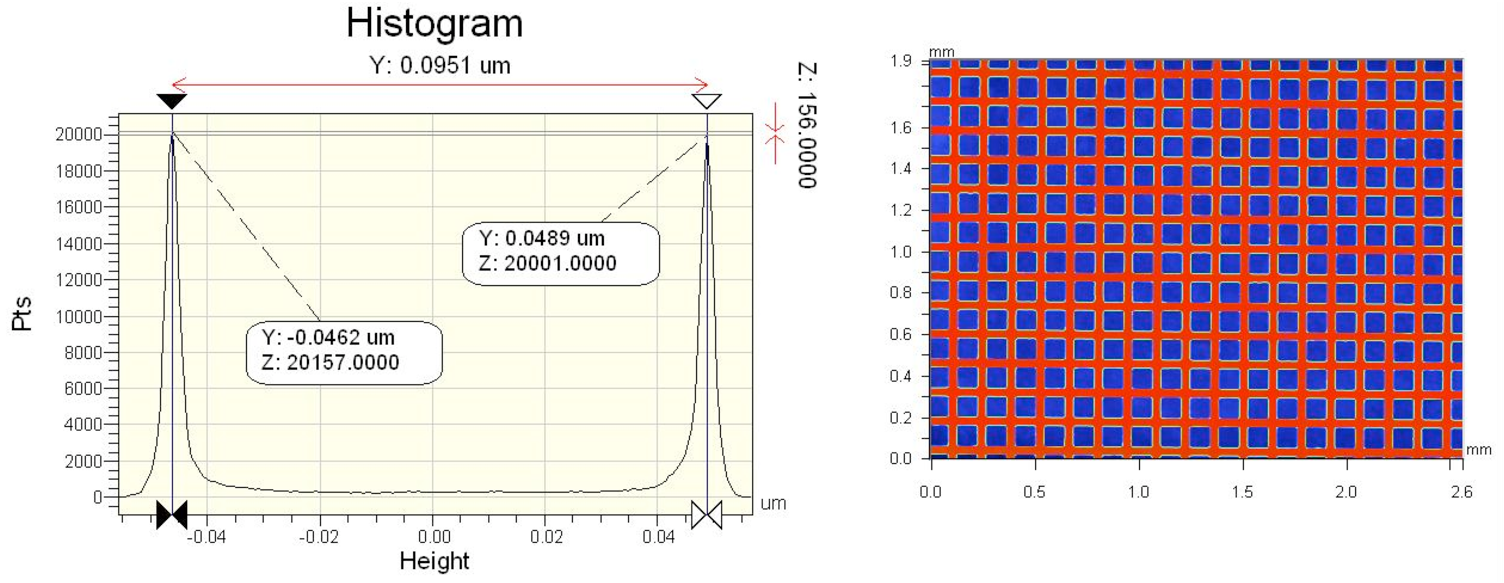
\includegraphics[width=1.0\columnwidth]{figs/VS20fineGapCrop.pdf}}
\caption{Veeco optical profiler surface plot and histogram for part VS20 in the fine pattern section\label{figVS20pattern}.  The four inch diameter VS20 is comprised of two thick silicon wafers.  We patterned three meshes with coarse, medium, and fine boxes, each with 50\% fill factors.  The depth was 95 $\pm$ 5 nm as indicated by the well-separated peaks in the Veeco profilometry histogram.  The Veeco was operated in PSI mode.  The purpose for these patterns was to have gaps of known dimensions against which we could test the optical metrology technique we describe in this paper.  The technique can reveal the axial extent and fill factor of an embedded gap.  }
\end{figure}


\begin{table}[h!]
\caption{UTexas Si bonding experiments \label{tabbondexper}}
\begin{center}
    \begin{tabular}{ c c c c c c}
    \hline
    Name & Diameter & Thickness & Pattern Type & Pattern Depth & Notes \\ 
    -  & mm & mm & - & nm & - \\ 
        \hline
    HA1     & 75   & $10$ $\times$ 2& None & - & \\
    VG01   & 100 &$1$ $\times$ 2 & None  & - &  \\
    VG02   & 100 & $3.3$ $\times$ 2 &  None  & - &  \\
    VG03   & 100 & $3.3$ $\times$ 2 &  Hole \&Petal & 4000$\pm$200 & See Fig. \ref{figVG03pattern}\\    
    VG04   & 100 & $1$ $\times$ 2 &  Patchwork Islands & 15$\pm7$ & \\
    VG07   & 100 & $1$ $\times$ 2 &  mesh C, M, F & 12$\pm7$ & \\ %see email from Victor on 5/16/13
    VG08   & 100 & $1$ $\times$ 2 &  mesh C, M, F & 12$\pm7$ & \\ 
    VG09   & 75   & $1$ $\times$ 2 & mesh C & 49 $\pm$6 & \\
    VG15   & 100 & $0.8$ $\times$ 2 &  mesh C, M, F  &14 $\pm$2 & \\
    VS20   & 100 & $0.8$ $\times$ 2 &  mesh C, M, F & 95 $\pm$5 & See Fig. \ref{figVS20pattern}\\
    \hline
    \end{tabular}
\end{center}
\end{table}


\begin{table}[h!]
\caption{Patterned gap properties \label{tabPatternFills}}
\begin{center}
    \begin{tabular}{ c c c c }
    \hline
    Pattern name & fill factor & minimum feature size & bulk description \\ 
    - & \% & $\mu$m & - \\ 
    \hline
    Hole & 100 & - & 25 mm diameter hole \\     
    Petal & $\sim1$ & $\sim$2000 & long petal lines, Fig. \ref{figVG03pattern} \\         
    Mesh F & 50 & 40 &  100 $\mu$m square holes, Fig. \ref{figVS20pattern}\\ 
    Mesh M & 50 & 200 &  500 $\mu$m square holes\\ 
    Mesh C & 50 & 620 &  1500 $\mu$m square holes\\     
        \hline
    \end{tabular}
\end{center}
\end{table}

\section{Substrate preparation}
We cleaned the surfaces before bonding to minimize the interfacial particle density.  The surface roughness was typically about 2 nm, as measured with a Veeco NT9100 Optical Profiler.  We measured the large scale surface flatness of the pucks.  The Fisba2 interferometer has a 2 inch diameter beam at $\lambda=$632.8 nm.  We found a typical peak to valley surface flatness of 2 waves over the central 2 inch diameter.  We prepared the substrates with standard cleaning procedures of solvents in a megasonic.  We then applied MHz frequency oxygen plasma ashing.  We soaked the wafers in DI water then dried with an N$_2$ gun.  We pressed the Si substrates together from the center to the outside.


\section{Measurement strategy, conditions, and details}
We took transmission spectra of bonded Si wafers and pucks, and double side polished Si reference wafers. The spectrophotometer is a Agilent Cary 5000 UV-Vis-NIR.  The typical measurement settings and tool performance are listed in Table \ref{tab:Cary5000pars}.  More details about the tool are available at the vendor's website.  Briefly, the tool has a double monochromator.  The double monochromator feature reduces scattered light.  The vendor reported linearity exceeds 40 dB.  

The Cary 5000 has four operation modes: single front, single back, double, and double reverse.  We experimented with single front and double modes.  Double mode takes a reference spectrum simultaneously to the target spectrum.  In both single and double beam mode, a baseline scan is taken with no sample in the measurement holder.  The baseline spectrum is the raw spectral response of the system.  We automatically divide sample spectra by the baseline spectrum.  In single beam mode, the baseline measurements must be repeated about every half hour.  We estimated the uncertainty and measurement repeatability of single and double modes in the following way.  We computed the RMS error and measurement repeatability in a single measurement by computing the standard deviation of a spectrum taken immediately after a baseline scan with no sample present.  The predicted mean level should naturally be 100\%.  We found that the mean value in single mode drifted by about 0.2\% over several measurements.  The standard deviation of the featureless spectrum was typically 0.02\% from point to point, with some portions of the spectrum demonstrating increased variance, perhaps attributable to atmospheric absorption; we list the wavelengths of instrumental artifacts and above-average variance in Table \ref{tab:Cary5000pars}. In double beam mode, the spectrograph performance was much better.  We put a double side polished (DSP) Si wafer in the reference beam, and no sample in the target beam during the baseline scan.  In this way the transmission spectrum of a target Si wafer is automatically normalized.  The double beam mode effectively divides out the 0.2\% drift in the mean transmission level attributable to lamp drift, as seen in single beam measurements.  In double beam mode, the drift in mean transmission level is merely 0.02\%.  These values are accurate for measurements over a half hour timescale or less.

The choice of spectral sampling was straightforward.  The spectral sampling was 2.0 nm.  The spectral resolution was 5.0 nm, the lowest spectral resolution the Cary5000 offers.  We expect smoothly varying spectral features for all conceivable interface gaps in Si bonded wafers.  Specifically, Fabry-P\`erot fringes attributable to interfacial gaps in bonded Si will be well-sampled with 5 nm spectral resolution, so long as the interface gap is less than $\sim$100 $\mu$m.  Such large gaps would be easily detectable by other means, like IR imaging.

\begin{table}[h!]
\caption{Summary of Cary 5000 Measurement parameters \label{tab:Cary5000pars}}
\begin{center}
\begin{tabular}{ c c }
\hline
        Parameter (Units) & Value \\ 
\hline
        Spectral sampling interval (nm) & 2.0$-$10.0 \\
        Spectral resolution (nm) & 5 \\
        Time per sample (s) & 0.1 \\
        Available measurement range (nm) & 175-3300 \\
        Typical measurement range (nm) & 1000-2500 \\
	Single mode RMS  (\%) & 0.02 \\
	Double mode RMS  (\%) & 0.002 \\
	Typical Single mode mean drift (\%) & 0.20 \\
	Typical Double mode mean drift (\%) & 0.02 \\
	No beam dark signal (\%) & 0.03 \\
 	Beam size (mm $\times$ mm) & $2 \times 8$ \\
	Wavelengths of instrumental artifacts (nm) & - \\
        		 & 1200 \\
		 & 1350 \\
		 & 1360-1450\\
		 & 1850 \\
		 & 1800-1950 \\
		 & 2000 \\
        Vendor-reported linearity range (dB) & $>40$ \\
        Directly measured linearity range (dB) & $>24$ \\
    \hline
    \end{tabular}
\end{center}
\end{table}


\subsection{IR bubble detection and limitations}

We looked for the indication of large gaps detectable as ``IR bubbles'' \cite{1992JEMat..21..669M} with IR imaging.  The detector was an IR Vista $\alpha$NIR infrared focal plane array, with 312 $\times$ 252 pixels, with 30 $\mu$m square pixels.  We used a 50 mm F/2 lens, with a fiber optic white light illumination source.  We estimate that the lamp-detector combination was sensitive to wavelengths in the range 1.1-1.6 $\mu$m.  The field of view sub-sampled the 4 inch diameter wafers, so we dithered the sample.  No effort was made to flat field the detector, so copious detector non-uniformities and vignetting are present in our images.  It was easy to detect IR bubbles despite the detector artifacts since the bubbles translate with the wafer during dithering.  We detected IR bubbles in all 3 of the bonded Si pucks on which we recorded IR images.  The bubble areal density varied from about 4 per 100 mm diameter bonded wafer pair to over 20 per bonded wafer pair.  Naturally, the unbonded DSP wafers show no such IR bubbles, which are entirely attributable to the gaps between bonded substrates as discussed in the literature (see Section \ref{secHistory}).  Figure \ref{IRbubble} shows an example of one of the IR bubbles in which several bright and dark fringes are clearly discernible.  No attempt at quantitative measurement was made on the IR images due to evidence that the detector is non-linear.  The morphology was clear regardless of the detector response.  


\begin{figure}[htbp]
\centerline{\includegraphics[width=.8\columnwidth]{figs/IR_bubble.pdf}}
\caption{Photo of part VG09 with transmission image of a bubble highlighted\label{IRbubble}.  The right side photo shows the 75 mm diameter wafer with blue Sharpie rectangles indicating the position of different spectral measurements (as detailed in the next section).  The yellow circle in the photo highlights the outline of the location of an IR bubble we detected.  The bubble shows $\sim2$ fringes over the effective wavelength range 1.1-1.6 $\mu$m.  This fringe pattern is consistent with a gap comparable to this measurement wavelength.  The pointlike measurement artifacts, Sharpie marker, and vignetting are perceptible in the raw IR image.  Our interpretation of the IR bubbles is robust against these artifacts.  The area surrounding the IR bubble appears to be mostly devoid of large (wavelength-scale) gaps, since the transmission is fairly uniform, and consistent with the brightest fringe of the IR bubble.  }
\end{figure}


\section{Results of infrared spectroscopy of bonded Si pucks}
\label{secResults}
In this section we describe the spectroscopy of bonded Si pucks.  In some instances IR imaging was available and was leveraged to target or avoid locations demonstrating IR bubbles.  In other cases the IR imaging was not available or ignored, and spectra were taken at random positions on the wafer surface.  

% Table of experiments
\begin{table}[h!]
\caption{Cary5000 Experiment Log \label{tabExperiments}}
\begin{center}
    \begin{tabular}{c c c c c c c}
    \hline
	Date &  Mode  & $\Delta \lambda$ & SBW & Sampling & \# of spectra & Sample IDs \\
	\emph{mm/dd/yyyy} &  -  & nm & nm & nm & - \\
%     \hline		
%	02/04/2013 & ? & ? 				& 5.0 & 10.0 &  16 &   -  \\
%     \hline		
%	02/06/2013 & ? & ? 				& 5.0 & 10.0 &  16 &   -  \\	     
     \hline		
     	02/18/2013 & Single & 1000$-$2500 & 5.0 & 10.0 &  16 &   -  \\
     	                   &            &                       &       &         &    4 &  Baseline\\	
     	                   &            &                       &       &         &    1 &  VG01\\
	                   &            &                       &       &         &    4 &  VG02\\	                   
	                   &            &                       &       &         &    2 &  VG03\\	                   
	                   &            &                       &       &         &    2 &  VG04\\
	                   &            &                       &       &         &    2 &  VG05\\	                   
	                   &            &                       &       &         &    2 &  VG06\\
    \hline
%	05/02/2013 & Single & 1000$-$2500 & 5.0 & 5.0  &  30 &   -  \\
%     	                   &            &                       &       &         &    12 &  Baseline\\	
%     	                   &            &                       &       &         &    18 &  Other\\
%    \hline
	05/03/2013 & Single & 1000$-$2500 & 5.0 & 5.0  &  28 &   -  \\
     	                   &            &                       &       &         &    8 &  Baseline\\	
     	                   &            &                       &       &         &    1 &  VG05\\ %Consider replacing VG05 with "DSP reference sample"  or something
     	                   &            &                       &       &         &    6 &  VG03\\
     	                   &            &                       &       &         &    13 &  Other\\ %These had to do with beam size experiments
    \hline
	06/07/2013 & Mix & 1000$-$2500 & 5.0 & 5.0  &  43 &   -  \\
	                   &            &                       &       &         &    11 &  Baseline\\	                   
	                   &            &                       &       &         &    9 &  VG05\\	                   
	                   &            &                       &       &         &    7 &  VG07\\
	                   &            &                       &       &         &    6 &  VG08\\
	                   &            &                       &       &         &    4 &  HA1\\
	                   &            &                       &       &         &    6 &  other\\ % These are mostly just baselines without automatic division
    \hline
	08/02/2013 & Single & 1000$-$2500 & 5.0 & 2.0  &  17 &   -  \\	
	                   &            &                       &       &         &    3 &  Baseline\\
	                   &            &                       &       &         &    4 &  VG05\\	                   
	                   &            &                       &       &         &    2 &  VG15\\
	                   &            &                       &       &         &    2 &  VS20\\
	                   &            &                       &       &         &    6 &  VG09\\
    \hline
    	09/11/2013 & Double & 1000$-$2500 & 5.0 & 2.0  &  20 &   -  \\	                   
	                   &            &                       &       &         &    1 &  Baseline\\
	                   &            &                       &       &         &    14 &  VS21\\	                   
	                   &            &                       &       &         &    5 &  Blank\\ %This is really the same as a baseline
    \hline
    	09/16/2013 & Double & 1000$-$2500 & 5.0 & 2.0  &  21 &   -  \\
	                   &            &                       &       &         &    2 &  Baseline\\
	                   &            &                       &       &         &    7 &  VG07\\	                   
	                   &            &                       &       &         &    4 &  VG05\\	
	                   &            &                       &       &         &    4 &  VG12\\
	                   &            &                       &       &         &    2 &  VG15\\	                   
	                   &            &                       &       &         &    2 &  VG08\\
    \hline
    \end{tabular}
\end{center}
\end{table}



\subsection{Constructing the predicted transmission}
We constructed the predicted transmission in the following way.  If IR imaging was unavailable, our optimistic prior belief was simply that the bond should be perfect and indistinguishable from a solitary DSP Si wafer, (i.e. 100\% relative transmission).  For the cases where we had bored gaps of known dimension and fill factors we could predict the transmission with the Fabry-Perot machinery described in section \ref{secTheory}.  Specifically we apply Equation \ref{eqFP}.  For non-unit fill factor, we simply average 100\% transmission with the predicted gap transmission, weighted by the estimated fill factor listed in Table \ref{tabPatternFills}.  No attempt was made to verify the delivered fill factor, but since high precision lithographic processes were employed, we assume the delivered fill factor is equal to the designed fill factor with no uncertainty.  The depth of the meshes has an associated uncertainty listed in Table \ref{tabbondexper}.  We incorporated the uncertainty in the mesh depth in the following way.  We computed the transmission curve for the 1$\sigma$ lower and upper bounds, and plot a filled band marked as the prediction band.  The uncertainties in the mesh depths were low enough that the band spread includes all intermediate lines of predicted transmission between plus and minus 1$\sigma$.  In cases where the IR imaging was unavailable the mesh position was only coarsely known, so our prediction band had to incorporate our uncertainty about whether or not our measurement beam was on or off or overlapping the mesh border.  If the beam was off the mesh we assumed 100\% relative transmission, so we simply set the lower bound of the predicted transmission to the equivalent of a zero gap.  

\subsection{Spectra of pucks with known gap sizes}
Figures \ref{VS21specm1} to \ref{VS21specf1} show examples of the predicted and measured IR spectra.  Figure \ref{VS21specm1} shows an example spectrum in which the measurement is consistent with the prediction for a gap with the known conditions.  Meanwhile, Figure \ref{VS21specf1} shows a spectrum in which the measurement marginally exceeds the prediction (by about $\sim 2 \sigma$).  Other parts show less consistency with the prediction.  A complete description of the diversity of the measured spectra requires an appeal to optical phenomena beyond the scope of this paper.  Briefly we classify the diversity of measurements into the categories laid out in the table below.  

\begin{figure}[htbp]
\centerline{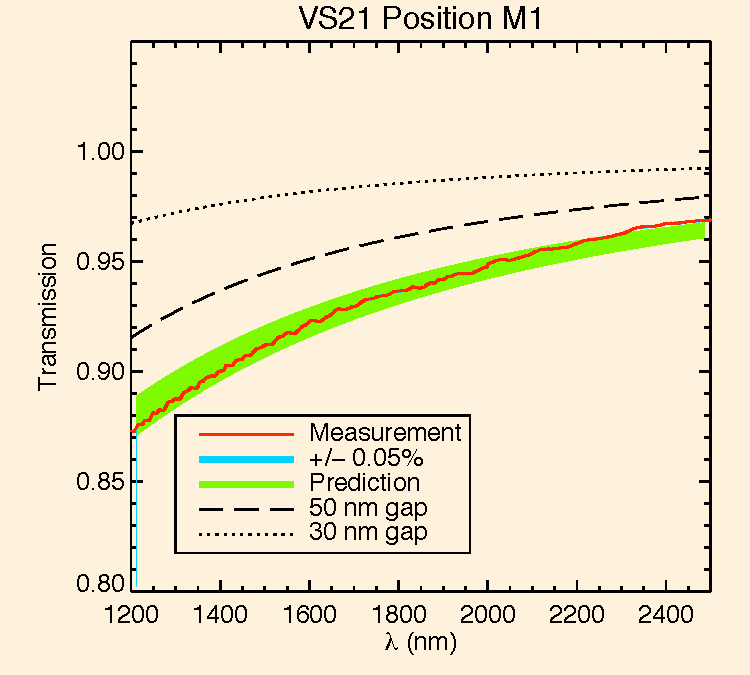
\includegraphics[width=.8\columnwidth]{figs/20130911_VS21posM1}}
\caption{IR transmission spectrum of VS21 (M1) showing consistent gap\label{VS21specm1}.  Example spectrum through part VS21 at a position through the mesh gap of known dimensions.}
\end{figure}

\begin{figure}[htbp]
\centerline{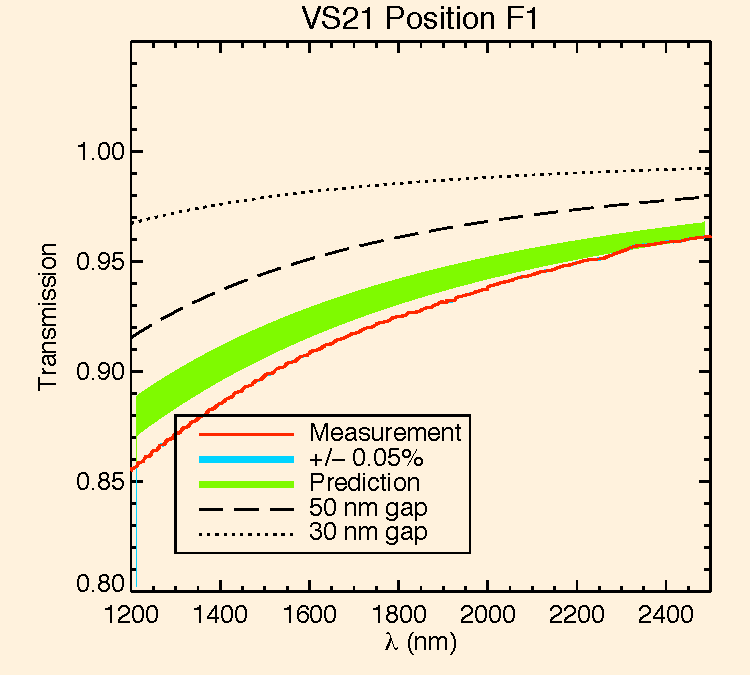
\includegraphics[width=.8\columnwidth]{figs/20130911_VS21posF1}}
\caption{IR transmission spectrum of part VS21 (F1) showing evidence for an excess gap\label{VS21specf1}.  The spectrum was taken at a position through a mesh gap of depth 95 $\pm$5 with 50\% fill factor.  The predicted spectrum lines up with the measurement to within the measurement and model uncertainties.}
\end{figure}


\begin{table}[h!]
  \caption{Interpretation of the diversity of IR spectra \label{tabInterpretation}}
  \begin{center}
    \begin{tabular}{ |p{8cm}| p{8cm} | p{2.2cm} |}
    \hline
    Appearance of spectra & Interpretation & Exemplars \\
    \hline
    Measurement within the prediction band & Life is good & VS21-M1, Figure \ref{VS21specm1}, VG15, VG07\\
    \hline
    Measured spectrum below the prediction band but shape is similar & Gap was slightly larger than predicted or bonding was incomplete& VS21-F1, Figure \ref{VS21specf1}, VS09, VG15, \\
    \hline
    Measured spectrum above the prediction band but shape is similar & Gap was slightly smaller than predicted & VS21-M2\\
    \hline
    Measured spectrum exceeds DSP reference puck & unanticipated anti-reflection coating on the surface of the Si sample (e.g. Sharpie marker residue) & VG08\\
    \hline
    High frequency, low amplitude wiggles superimposed upon smooth underlying trend & Large, unanticipated gap, with a small fill factor  & VS21-C3\\   
     																			     & wavelength dependent diffraction from the mesh patterns & VS21-C3\\       
     																			     & measurement artifact  & VS21-C3\\       												
    \hline
    Non-unit transmission constant with wavelength (gray spectrum) & Artifact of measurement- vignetting of beam, absorptive coating, zero-point drift & VS21-C4 \\
    \hline
    Completely different spectrum than anticipated with low absolute transmission & Large, inhomogeneous gap consistent with an IR bubble & VG09 \\
    \hline
    \end{tabular}
  \end{center}
\end{table}

A key result of this work is to show that gaps of known dimensions are recovered in our spectroscopy.  The cases in which predicted spectroscopy differs from measurement are due to either a bona-fide detection of a gap above and beyond the implanted gap, or some measurement artifacts.  In the next section we address mitigation of artifacts.

\subsection{Mitigation of measurement artifacts}
The principle artifacts and their interpretation are listed in Table \ref{tabInterpretation}.  We mitigated the artifacts in the following ways.  For the Sharpie marker behaving as an anti-reflection (AR) coating, we simply removed the sharpie with IPA.  We have mostly been able to rule out wavelength-dependent diffraction from the mesh pattern as a measurement artifact, since the beam size is large and the angular spread of diffraction from the mesh pattern would be much smaller than the spread of the beam.  Still, to remove this concern, we moved to using the coarse mesh rather than the medium or fine meshes, when possible.  We saw no difference in the bond quality surrounding the medium or fine meshes, which is consistent with results from the literature \cite{1992JEMat..21..669M}.  Specifically, the gas pressure of bonded wafers grows as the fill factor of gaps decreased.  In other words, what matters is the fill factor of gaps, not their relative sizes.  Since the fine, medium, and coarse meshes had the same fill factors, we anticipate no difference in the pressure of the gaps, and therefore no difference in the bonding properties.

\subsection{Non-normal incidence angles}
For the vast majority of applications, normal incidence performance is the quantity of interest.  The technique laid out in this paper outlines an approach for measuring the gap size of bonded Si wafers at normal incidence.  In principle, from there the performance at non-normal incidence can be worked out either by simulation or calculation.  Here we briefly motivate the challenge of experiment and simulation at non-normal incidence.  

\begin{figure}[htbp]
\centerline{\includegraphics[width=0.95\columnwidth]{figs/Sibondedprismcartoon.pdf}}
\caption{Schematic of a bonded Si immersion grating\label{figSiPrism}.  }
\end{figure}

Our final application that motivated this project is to make diffraction gratings on the hypotenuse of a silicon prism.  The diffraction occurs inside the silicon material and is dispersed and reflected back along its path.  This configuration is called an immersion grating.  Figure \ref{figSiPrism} shows a schematic of the geometry of our bonded Si immersion grating.  Our group has made monolithic immersion gratings for over a decade, but challenges in processing large (30 mm thick) Si wafers motivated an approach of patterning and processing thin (1-10 mm thick) Si wafers, and then bonding them to shaped and polished prisms.  This technique has been pioneered at SRON \cite{2012SPIE.8450E..2TV}.  In Figure \ref{figSiPrism} we show an example with a 10 mm thick Si puck bonded to a 25 mm thick, precision cut, shaped, and polished Si prism.  The group at SRON has patterned Si immersion echelle gratings on commercial thin  ($< 1$ mm) Si wafers.  Thin wafers have the drawback that they are conformal, so total-thickness-variations (TTV) directly translate into surface optical aberrations\cite{2012SPIE.8450E..2TV}.  

The consequence of our immersion grating design is a non-normal incidence interface in double pass.  In this case, the Fabry-P\'{e}rot framework developed here fails to predict the spectrum of the interface loss attributable to a finite albeit small (few nm) gap.  Specifically, complete internal reflection and evanescent waves will matter at large incidence angles, and the incoherent matrix technique is no longer accurate.  Polarization effects are important.  We do not have a mechanism for evaluating the bond performance until the final device is completed and its wavelength-dependent transmission is measured.  We can detect the performance degradation on final devices in the following nuanced way.  We will measure the efficiency of the bonded Si immersion grating as a function of both wavelength and angle.  Our group built a custom tool to make these measurements- the Custom Robotic Order, Wavelength, and Blaze Angle Recorder (CROWBAR) \cite{2012SPIE.8450E..2SG}.  Figure 3 in \cite{2012SPIE.8450E..2SG} shows the directly measured spectrum of a monolithic immersion grating.  Notably, the spectrum in Figure 3 in \cite{2012SPIE.8450E..2SG}  shows dozens of blaze peaks where the efficiency should be maximized.  A perfectly contacted Si$-$Si direct bonded optic would have identical performance to a monolithic counterpart.  Bonded immersion gratings with finite gap sizes will superimpose a wavelength dependent transmission loss on top of the blaze peaks.  In this way, the presence or absence of deleterious gaps can be identified in final immersion gratings.  One drawback of this approach is that gaps can only be identified after the costly process of producing the final optical device.  Large gaps identified this late in the game could render the costly optic useless, both in terms of efficiency and wavefront performance.  Our group is exploring the effectiveness of high-temperature annealing to eliminate interfacial gaps in completed devices.


\subsection{Spectra of pucks with no implanted gap}
We have shown that the IR spectroscopy technique combined with the Fabry-P\'{e}rot framework provide accurate knowledge of the gap size.  In the cases where we expected no gap (i.e. perfect Si-Si bond), we have seen spectra consistent with 100\% transmission relative to a DSP Si wafer.  In other cases we have seen evidence for gaps, which is simply an indication that the bonding process introduces gaps.  In a followup paper we will describe ways to mitigate bond formation in bonded Si pucks.

\section{Conclusions}
We have shown a method for indirectly measuring the size of gaps in bonded Si wafers.  The technique broadly applies to any compound Si optics measured at normal incidence.  We showed lab IR spectra with consistent predictions, and addressed ways to mitigate measurement artifacts. 

\appendix

\section{Appendix: X-ray Computed Tomography}
We acquired x-ray computed tomography of sample VG03.  The measurement details are listed in Table\ref{tab:tablenum4}.

\begin{table}[h!]
\caption{Summary of X-ray CT measurements for VG03 \label{tab:tablenum4}}
\begin{center}
    \begin{tabular}{ll}
    \hline
    \emph{Parameter (Units)} & \emph{Value} \\ 
    \hline
    Instrument& Xradia MicroCT \\
     Objective & 0.7X \\
    Accelerating voltage (kV) & 100 \\
        Power (W) & 10 \\
        Acquisition time (s) & 3.5 \\
        Number of views & 2521 \\
        Total slices & 469 \\
        Field of view diameter (pixels) & 988 \\
        Voxel lateral pixel resolution ($\mu$m) & 38.02 \\
        Estimate field of view (mm) & 37.5 \\
        Voxel axial pixel resolution ($\mu$m) & 0.5 \\
        Scan date & 2013 August 8 \\
        Sample thickness (mm) & 6.6 \\
    \hline
     \end{tabular}
\end{center}
\end{table}

The axial resolution of the X-ray CT system is about 500 nm, which is much larger than the small ($\sim$ 15$-$90 nm) patterned gaps on many of our bonded samples.  Part VG03 has a cylindrical patterned gap with a $\sim$20 mm diameter and 4000 nm height.  We expected to see the cylindrical gap in about 8 resolution elements, given that the pattern was centered in the 25 mm diameter field of view.  We saw a circular feature that extended over 297 pixels, which corresponds to 11.3 mm, assuming the voxel lateral dimension from the table above, which is reported in the X-ray CT lab measurement details.  The feature...


\section{Incoherent Multiple Reflections Transfer Matrix Method}
\label{sec:Append-IMRTMM}

The wave transfer matrix method is described in detail in chapter 7 by Saleh and Teich in ``Fundamentals of Photonics'' \cite{2007fuph.book.....S}.  Briefly, their technique is to assemble a 2$\times$2 scattering matrix $\boldsymbol{S}$ which has the elements:
\begin{eqnarray}
\boldsymbol{S} = \left(
\begin{array}{cc}
 t_{12} & r_{21} \\
 r_{12} & t_{21} \\
\end{array}
\right)
\end{eqnarray}
Where $t$ and $r$ stand for transmission and reflection respectively.  The order of subscripts is the order of origin and destination of the wave in regards to the interface, so we know something about the direction of the wave and how it got there.  The $\boldsymbol{S}$ matrix encapsulates all the information we need to know about how light waves interact with the interface.  The real power of the matrix technique comes from a cousin of the scattering matrix, the so-called wave transfer matrix, $\boldsymbol{M}$.  The matrix $\boldsymbol{M}$ has the convenient property that its output can be used as the input for another matrix.  In other words, the input vector to $\boldsymbol{M}$ is made of the left and right moving components directly before the interface; the outputs are the left and right moving components directly after the interface:
\begin{eqnarray}
\left(
\begin{array}{c}
 U_2^{(+)} \\
 U_1^{(-)} \\
\end{array}
\right)=\boldsymbol{S} \left(
\begin{array}{c}
 U_1^{(+)} \\
 U_2^{(-)} \\
\end{array}
\right) \\
\left(
\begin{array}{c}
 U_2^{(+)} \\
 U_2^{(-)} \\
\end{array}
\right)=\boldsymbol{M} \left(
\begin{array}{c}
 U_1^{(+)} \\
 U_1^{(-)} \\
\end{array}
\right)
\end{eqnarray}

The elements of $\boldsymbol{S}$ and $\boldsymbol{M}$ are related to each other by geometric transformations\cite{2007fuph.book.....S}.  Much of the literature on the transfer matrix method deals with applications related to thin films, in which the wavelength is comparable to the size of the dielectric layer.  For thin films the vector components $U_{i}$ represent the complex amplitudes of the electromagnetic waves.  The polarization state can be encapsulated in scattering matrix components\cite{2007fuph.book.....S}.  The intensities of the emergent spectrum can be computed from the absolute square of the complex amplitudes.  For thick films, the vector components are the intensities of the emergent spectrum, since waves are incoherent.  \cite{2002ApOpt..41.3978K} work out the general transfer-matrix method for optical multilayer systems with incoherent interference.  The key idea for the incoherent transfer matrix method approach is to populate a scattering matrix with elements equal to the (wavelength dependent) transmitted $T_i$ and reflected $R_i$ intensities of an interface or set of interfaces that act together.  Then, use the geometric transformations to construct the $\boldsymbol{M}$ matrix.  

The matrix for the Fabry-P\`erot etalon is calculated in the following way.  The first key idea is that I had to treat the entire air gap as an abstraction, a Fabry-P\`erot etalon.  We don't need to bother to consider the microscopic coherent interactions with the etalon transmission, all of that information is encapsulated in these equations for a Fabry-P\`erot etalon.

\begin{eqnarray}
 \delta = \frac{2\pi}{\lambda}2d \\
  F \equiv \frac{4R}{(1-R)^2} \\
 T_e = \frac{1}{1+F\sin^2(\delta/2)}  \label{eq:FabPerot}
\end{eqnarray}

with $\lambda$ the vacuum wavelength, $R$ the Fresnel reflection of silicon, and $F$ the coefficient of finesse.  The coefficient of finesse $F$ and the phase $\delta$ are the two parameters of the Fabry-P\`erot etalon.  The coefficient of Finesse encapsulates the Fresnel reflection and depends only on the Si refractive index which has a minute wavelength (and temperature) dependence.  The phase depends on the wavelength $\lambda$ and $d$ the air gap spacing: $\delta=\frac{2\pi}{\lambda}2d$ .  We assume the etalon is lossless, i.e. the etalon has no absorption $T_e+R_e=1$.  So the incoherent scattering and transfer matrices for the etalon are:

\begin{eqnarray}
\boldsymbol{S_e}&=&\frac{1}{1+F\sin^2{\delta/2}} \left(
\begin{array}{cc}
1 & F \sin ^2(\delta/2) \\
F \sin ^2(\delta/2) & 1 \\
\end{array}
\right) \nonumber \\
\nonumber \\
\boldsymbol{M_e}&=&\left(
\begin{array}{cc}
 1-F \sin ^2(\delta/2) & F \sin ^2(\delta/2) \\
 -F \sin ^2(\delta/2) & 1+F \sin ^2(\delta/2) \\
\end{array}
\right)
\label{eqn:EtalonMatrix}
\end{eqnarray}

I assembled the matrix for the Air-Si Fresnel interface in the following way.  First it is important to note that the matrix is the same whether the transmission is from Si to air or air to Si.  This reciprocity is not necessarily true for the complex amplitudes matrix, but our approach employs intensities not complex amplitudes.  The Fresnel interface is lossless.  The transmission and reflection are given by the Fresnel equation for normal incidence:
\begin{eqnarray}
T_n&=&\frac{4n_{Si}}{(n_{Si}+1)^2} \\
R_n&=&\frac{(n_{Si}-1)^2}{(n_{Si}+1)^2} \label{eq:FresnelTrans}
\end{eqnarray}
For clarity I will drop the subscripts from $n_{Si}$, since we have already set $n_{air}=1$ and there are no other dielectric interfaces to think about.  So the scattering and transfer matrices for the air-Si Fresnel boundary are:

\begin{eqnarray}
\boldsymbol{S_n}&=&\frac{1}{(n+1)^2} \left(
\begin{array}{cc}
4n & (n-1)^2 \\
(n-1)^2 & 4n \\
\end{array}
\right)  \nonumber \\
\nonumber \\
\boldsymbol{M_n}&=&\frac{1}{4n}\left(
\begin{array}{cc}
 -n^2+6  n-1 & ( n-1)^2 \\
 -( n-1)^2 & ( n+1)^2 \\
\end{array}
\right)
\label{eqn:SiAirMatrix}
\end{eqnarray}

Finally, we cascade the matrices together to compute the net transmission through the stack of abstractions.  The result is a $2\times2$ transfer matrix: $$\boldsymbol{M_{net}}=\boldsymbol{M_n}\boldsymbol{M_e}\boldsymbol{M_n}$$  From the matrix transformation equations \cite{2007fuph.book.....S} we know $M_{22}=1/T$.  Taking the inverse of the bottom right element of $\boldsymbol{M_{net}}$, we get the transmission $T_{net}$ through the net optical device: 

\begin{eqnarray}
T_{net}=\frac{2 n}{1+ 2n F\sin ^2(\delta/2)+n^2} \label{eqn:FPmatTrans}
\end{eqnarray}

Compare equations \ref{eqn:FPmatTrans} and \ref{eq:FabPerot}.  The revised transmission has picked up a few factors of 2 and $n$.  While we are at it, let's compute the matrix for the scenario with no intermediate etalon: there are simply two Fresnel interfaces with which light interacts incoherently.  This scenario is the model for a single DSP reference puck. The revised matrix multiplication is simply $\boldsymbol{M_{DSP}}=\boldsymbol{M_n}\boldsymbol{M_n}$.  Taking the inverse of the $M_{22}$ element, we find: 
\begin{eqnarray}
T_{DSP}=\frac{2 n}{n^2+1}\label{eqn:EqofSummedSlab}
\end{eqnarray}
which is identical to the result obtained by directly summing the intensities from multiple reflections:
\begin{eqnarray}
T_{DSP}=T^2 \sum_{i=0}^{N}R^{2i} \label{eqn:multsum}
\end{eqnarray}

It is informative to isolate the effect of the gap by dividing the measured bonded wafer transmission by the transmission of a reference DSP Si part.  We call this normalized transmission the etalon transmission $T_{e}$:
\begin{eqnarray}
T_{e} = T_{net}/T_{DSP} \\
T_{e} = \frac{n^2+1}{2 n F \sin ^2(\delta/2)+n^2+1} \label{eqn:Tetalon}
\end{eqnarray}

\section{Appendix: High spectral resolution coherent interference of thin substrates}

Throughout this article we have assumed that $L >> \lambda^2 / \delta \lambda$, so that the interference of the substrate is safely incoherent.  Another way of stating this criterion is that the spectral bandwidth is large enough that high spectral frequency fringes average out in a composite spectrum of low spectral resolution.  If we relax this assumption so that the Si substrate thickness is comparable to or smaller than the coherence length, we would begin to observe high frequency fringes in the transmission spectra.  In this appendix section we work out the transmission spectrum for two scenarios.  First, we work out the case of a DSP Si wafer of thickness $L$, with no gap.  Second we work out the case of two bonded Si wafers of thicknesses $L_1$ and $L_2$.  For both cases we consider infinite spectral resolution, then convolve the spectra with a finite spectral resolution to show that the spectrum tends to that derived using an incoherent assumption.  

\subsection{DSP Si wafer at high spectral resolution}
The Fabry-P\`erot etalon transmission is given in Equation \# X (currently, 5).  What we want to evaluate is:
  
$$
 <T_e> = \lim_{\sin^2(\delta/2) \to 0.5} \frac{1}{1+F\sin^2(\delta/2)} \\
 <T_e> = \frac{1}{1+F/2}
$$



\bibliographystyle{osajnl}
\bibliography{AO_bondedSi}


%\begin{thebibliography}{99}

%% Do not include separate BibTeX files; if BibTeX is used,
%% paste the output (contents of .bbl file) here.

%\end{thebibliography}

\end{document}
